\documentclass[sigconf,nonacm]{acmart}

\usepackage{booktabs}
\usepackage{array}
\usepackage{amsmath}
\usepackage{graphicx}
\usepackage{enumitem}
\usepackage{multirow}

\graphicspath{{figures/}}
\settopmatter{printacmref=false}
\renewcommand\footnotetextcopyrightpermission[1]{}

\title[Complementary Cues for Tampering Localization]{Selecting Complementary Classical Cues for Image Tampering Localization}
\author{CSE 4883 Digital Image Processing Project Team}
\affiliation{\institution{Department of Computer Science and Engineering, United International University}\city{Dhaka}\country{Bangladesh}}

\begin{abstract}
Image-tampering detectors are usually specialized. A copy-move detector searches for repeated content, a JPEG detector searches for compression history, and a resampling detector searches for interpolation traces. A detector can therefore fail when an edit does not leave the trace it assumes. This paper studies cue selection rather than assuming a fixed detector set. We compare four classical candidates: SIFT-based duplicated-content matching, a JPEG recompression inconsistency cue, a periodic resampling cue, and an 8$\times$8 block-aligned anomaly cue. Each candidate produces a spatial evidence map. Map normalization, fusion weights, and the decision threshold are fitted on validation data only. A held-out pilot with 40 independent source identities selected JPEG history, resampling, and block-grid evidence, with validation weights 0.25, 0.25, and 0.50. The selected subset reached Dice 0.2062 on the pilot test split. The result is modest and varies by manipulation type, so it is reported as evidence about cue selection under the stated protocol, not as a universal authenticity claim. The repository records public-source provenance, source-disjoint manifests, detector timing, and failure conditions.
\end{abstract}
\keywords{image forensics, image tampering, copy-move detection, JPEG artifacts, resampling traces, cue fusion, localization}

\begin{document}
\maketitle

\section{Introduction}
Image tampering detection has two linked goals: decide whether an image contains an alteration and localize the altered region. The second goal is harder than image-level classification because the evidence is spatial and may be weak. A copied object may preserve the local appearance of the source image. A splice may leave a compression or interpolation mismatch. An object replacement may leave neither trace in a reliable form.

Classical forensic methods are useful because their evidence can be inspected and their assumptions can be stated. Their specialization is also a limitation. SIFT matching is suitable for duplicated content but does not measure JPEG history. JPEG ghost analysis is conditional on a useful compression history. Resampling analysis is conditional on interpolation. Combining such cues may help, but adding cues can also add redundant false positives and computational cost.

This paper asks a narrow and testable question: does a validation-selected subset of classical evidence maps improve localization over the strongest individual cue under a fixed data protocol? The study treats the candidate set as an experimental variable. It does not assume that three cues, or all available cues, are complementary.

Our contributions are fourfold:
\begin{enumerate}[leftmargin=*]
  \item a candidate-pool formulation that separates duplicated-content, compression, geometric, and block-aligned evidence;
  \item a validation-only subset and weight-selection protocol with explicit handling of unavailable cues;
  \item a reproducible implementation with source-disjoint manifests, deterministic stress transforms, machine-readable reports, and detector timing; and
  \item a measured pilot result that shows both the selected subset and its limitations instead of claiming universal superiority.
\end{enumerate}

\begin{figure}[t]
  \centering
  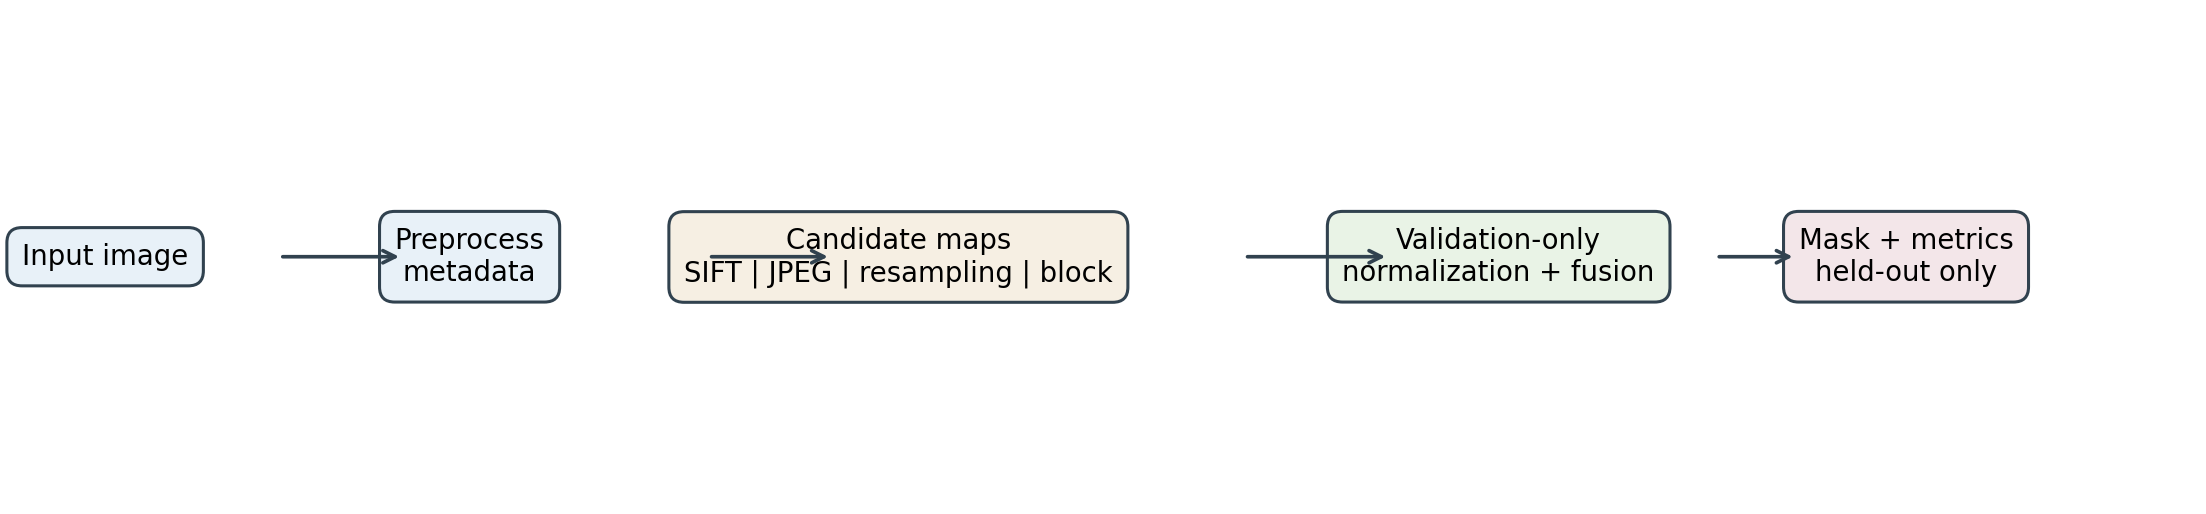
\includegraphics[width=\linewidth]{pipeline.png}
  \caption{Working order of the proposed study. Ground-truth masks are read only by the evaluation stage. Cue selection and score calibration are completed before the held-out test is opened.}
  \label{fig:pipeline}
\end{figure}

\section{Related Work}
\subsection{Duplicated content}
Fridrich et al. formulated copy-move detection as the search for repeated image regions \cite{fridrich2003}. Amerini et al. used SIFT correspondences and transformation recovery, motivating geometric verification before accepting a match \cite{amerini2011}. Christlein et al. showed that copy-move performance changes with image content and manipulation type \cite{christlein2012}. The COVERAGE database further demonstrates that natural images can contain similar genuine objects that resemble copied regions \cite{wen2016}. These works motivate both the SIFT candidate and the use of negative controls.

\subsection{Compression history and JPEG structure}
Farid's JPEG ghost method tests recompression responses at candidate quality factors and relates local error minima to prior JPEG compression \cite{farid2009}. Fan and de Queiroz studied compression-history identification and quantizer estimation \cite{fan2003}. Bianchi and Piva used block-grained JPEG artifacts for localization \cite{bianchi2012}. More recent JPEG-aware work treats compression as an experimental condition rather than a nuisance that can be ignored \cite{wang2022,verma2023}. Our JPEG candidate is therefore described as a pixel-domain recompression approximation, and our block candidate is described as a block-aligned anomaly heuristic.

\subsection{Resampling traces}
Popescu and Farid showed that interpolation can create periodic correlations that are detectable in local image regions \cite{popescu2005}. This evidence is mechanistically different from duplicated content and compression history, but it is conditional. An edit without resizing, rotation, or warping may not produce a measurable resampling trace. The survey by Qazi et al. places these cues within a broader passive-forensics taxonomy and supports reporting detector assumptions explicitly \cite{qazi2013}.

\subsection{Comparison with the proposed study}
Table~\ref{tab:related} states the relation between prior work and the present study. The contribution is not a new descriptor. It is an auditable selection experiment in which the smallest useful cue subset is measured under one fixed protocol.

\begin{table}[t]
\caption{Literature-to-method mapping.}\label{tab:related}\small
\begin{tabular}{p{0.19\linewidth}p{0.29\linewidth}p{0.42\linewidth}}
\toprule Evidence domain & Representative work & Use and boundary in this study \\
\midrule
Duplicated content & Fridrich et al.; Amerini et al.; Christlein et al. & SIFT matching with affine RANSAC. Tested against repeated natural structure; not treated as a general splice detector. \\
JPEG history & Farid; Fan and de Queiroz & Candidate-quality recompression response. Available only when JPEG history is preserved; implemented as an approximation. \\
JPEG block structure & Bianchi and Piva; Verma et al. & 8$\times$8 DCT and boundary anomaly. Ablation candidate because it may overlap with JPEG history. \\
Resampling & Popescu and Farid & Local periodicity screening. Interpreted as geometric-edit evidence, not universal tamper evidence. \\
Cue selection & This work & Validation-only subset ranking, held-out evaluation, availability tracking, and runtime reporting. \\
\bottomrule
\end{tabular}
\end{table}

\section{Research Questions and Study Design}
The study uses two research questions:
\begin{description}[leftmargin=!,labelwidth=1.2cm]
  \item[RQ1] Does fusion improve localization over the strongest individual cue under the same split and threshold-selection protocol?
  \item[RQ2] Which smallest cue subset provides the best validation score without relying on unavailable or redundant evidence?
\end{description}

The main hypothesis is conditional: cues from different evidence domains may reduce different error types, while two compression-related cues may be redundant. The hypothesis is tested by ablation, not asserted from detector names.

\subsection{Working order}
The experiment follows this order:
\begin{enumerate}[leftmargin=*]
  \item register sources, masks, manipulation type, format, and source identity;
  \item assign source identities to train, validation, and test before generating related variants;
  \item run every applicable candidate detector and record availability and runtime;
  \item fit map normalization, nonnegative weights, and threshold on validation data;
  \item rank every candidate subset by validation Dice, then by subset size and runtime;
  \item freeze the selected subset and evaluate it once on held-out data; and
  \item report results by manipulation type, stress condition, and failure mode.
\end{enumerate}

\subsection{Dataset provenance}
The controlled pilot uses deterministic source identities and known masks. Public-data support is prepared for CoMoFoD and COVERAGE. CoMoFoD provides original images, forged images, binary masks, and post-processing variants. COVERAGE provides original-forged pairs with duplicated and forged region masks and explicitly includes similar genuine objects. Official CoMoFoD examples are included for sanity checking, while quantitative benchmark evaluation requires the full licensed archive and its binary masks.

\begin{table}[t]
\caption{Data sources used or prepared for the study.}\label{tab:data}\small
\begin{tabular}{p{0.19\linewidth}p{0.24\linewidth}p{0.44\linewidth}}
\toprule Source & Role & Evidence boundary \\
\midrule
Controlled pilot & Weight and subset protocol & 40 independent seeds, four manipulation types, JPEG quality 88, known masks; pilot evidence only. \\
CoMoFoD examples & Detector sanity check & Official original/forged examples; no binary masks on the example page, so no localization score is reported. \\
CoMoFoD full release & Planned benchmark & Official archive contains binary masks and post-processing variants; local licensed extraction is required. \\
COVERAGE & Planned copy-move benchmark & Author-controlled archive with similar-genuine-object controls and region masks. \\
\bottomrule
\end{tabular}
\end{table}

\section{Method}
\subsection{Input standardization}
Each image is converted to RGB and grayscale representations. EXIF orientation is applied before analysis. The original format, original size, processed size, resize factor, and JPEG availability are stored in the detector result. JPEG-specific candidates are marked unavailable after a geometry-changing resize. An unavailable cue contributes no score and cannot contribute to fitted normalization statistics.

\subsection{Candidate cues}
\paragraph{Duplicated-content cue.} SIFT keypoints and descriptors are extracted. Descriptor matches are filtered by a ratio test and minimum spatial separation. An affine partial transform is estimated with RANSAC. Only sufficiently supported inliers produce evidence. The output map is formed from inlier points and their convex hulls, then smoothed. This map identifies repeated-content evidence; it does not identify all splices.

\paragraph{JPEG recompression cue.} For a JPEG input that has not been resized, the image is recompressed at a fixed set of quality factors. Local squared pixel error is aggregated over a window. The quality response and its local disagreement are converted into a normalized suspicion map. This implements the observable pixel-domain part of the JPEG-ghost idea, but it is not claimed to reproduce every DCT-domain detail of Farid's method.

\paragraph{Resampling cue.} A second-difference residual is calculated. Local FFT spectra are searched for strong noncentral periodic peaks. The local responses are smoothed and normalized. The output is interpreted as interpolation evidence. It is not expected to respond to every object replacement or splice.

\paragraph{Block-aligned cue.} The grayscale image is divided into 8$\times$8 blocks. High-frequency DCT energy and block-boundary differences are measured. Robust median/MAD scores produce a block-aligned anomaly map. This cue is an ablation heuristic and is retained only when it adds validation value beyond compression-history evidence.

\subsection{Normalization and fusion}
For cue $k$, validation percentiles $(a_k,b_k)$ define
\begin{equation}
  \widetilde{S}_k(x,y)=\operatorname{clip}\left(\frac{S_k(x,y)-a_k}{b_k-a_k},0,1\right).
\end{equation}
For the available cue set $A$, the equal-weight baseline is
\begin{equation}
  F_{\mathrm{eq}}(x,y)=\frac{1}{|A|}\sum_{k\in A}\widetilde{S}_k(x,y).
\end{equation}
The tuned variant uses nonnegative weights satisfying $\sum_{k\in A}w_k=1$:
\begin{equation}
  F(x,y)=\sum_{k\in A}w_k\widetilde{S}_k(x,y).
\end{equation}
If a cue is unavailable for one image, the active weights are renormalized over the remaining cues. A threshold produces the binary mask. The implementation records the selected weights, threshold, normalization values, availability, and runtime.

\subsection{Subset selection}
Every nonempty subset of the candidate pool is evaluated on validation data. A coarse simplex grid supplies candidate weights. The selection rule is lexicographic: maximize validation Dice, prefer the smaller subset within a tie, then prefer lower runtime. The test split is not used in this decision.

\subsection{Evaluation measures}
For prediction $P$ and ground-truth mask $M$, the study reports precision, recall, F1, IoU, and Dice. Runtime is reported per detector and for the complete pipeline. Public benchmark experiments will add paired bootstrap intervals for the difference between the selected subset and the strongest individual cue. Stress conditions include recompression, resizing, blur, and additive noise.

\section{Implementation and Results}
\subsection{Implementation}
The system is implemented in Python using OpenCV, NumPy, SciPy, Pillow, and scikit-learn-compatible numerical tools. The command-line entry point stores maps as NumPy arrays and writes JSON and static HTML summaries. The test suite contains detector, fusion, manifest, perturbation, and mask-geometry checks.

\subsection{Pilot protocol}
The pilot contains 40 independently seeded images: 10 copy-move, 10 splicing, 10 object replacement, and 10 geometric-edit samples. All images are saved as JPEG at quality 88. Four images per manipulation type are used for validation and eight for the held-out pilot test. The source identities are disjoint across the two splits. The pilot verifies the experimental workflow and exposes detector behavior; it is not a substitute for the complete public benchmark.

\subsection{Cue-subset result}
Validation selected JPEG history, resampling, and block-grid evidence with weights 0.25, 0.25, and 0.50. The full four-cue pool reached the same validation score but was rejected by the minimum-subset rule. Figure~\ref{fig:ablation} shows the leading subset comparison.

\begin{figure}[t]
  \centering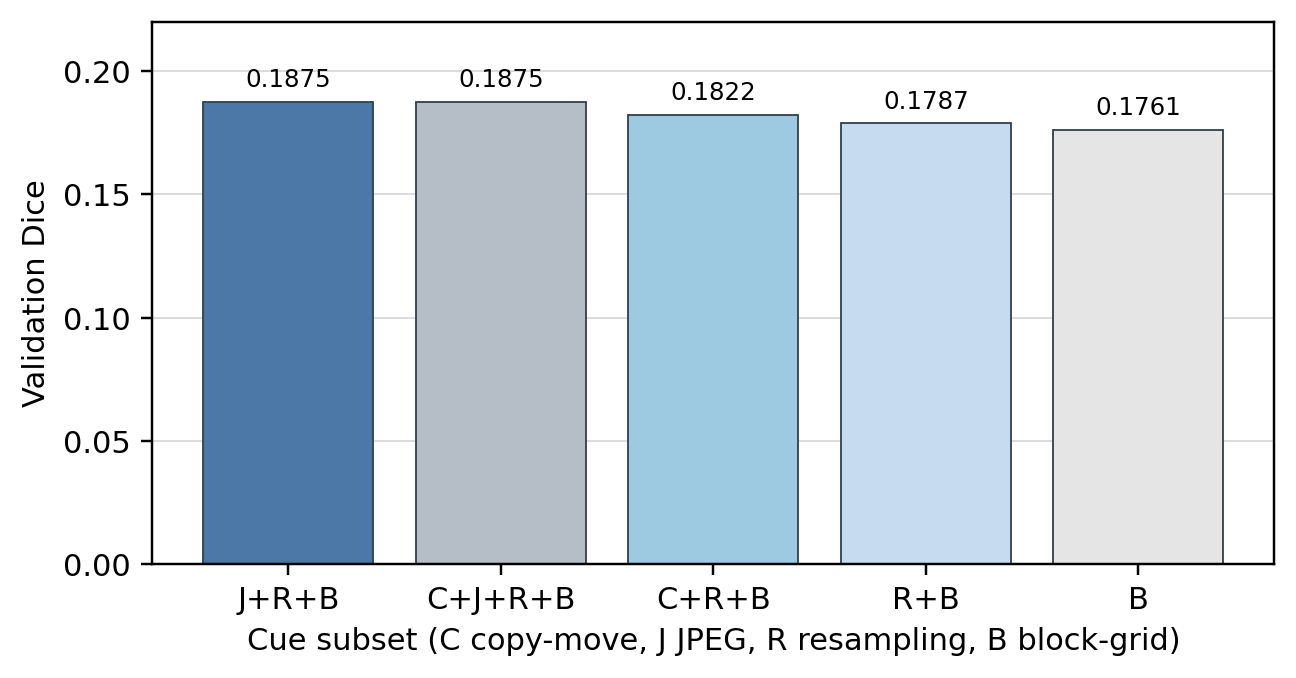
\includegraphics[width=0.96\linewidth]{pilot_ablation.png}
  \caption{Leading validation subsets in the controlled pilot. The full pool tied the selected subset, so the smaller subset was retained. This is a pilot ablation, not a benchmark comparison with published methods.}\label{fig:ablation}
\end{figure}

\begin{table}[t]
\caption{Pilot validation subset ranking.}\label{tab:ablation}\small
\begin{tabular}{lcc}\toprule
Subset & Validation Dice & Decision \\
\midrule
JPEG + resampling + block & 0.1875 & selected \\
Copy + JPEG + resampling + block & 0.1875 & tied; larger \\
Copy + resampling + block & 0.1822 & not selected \\
Resampling + block & 0.1787 & not selected \\
Block only & 0.1761 & not selected \\
\bottomrule\end{tabular}
\end{table}

\subsection{Held-out pilot result}
The selected subset obtained mean Dice 0.2062 on the held-out pilot. Figure~\ref{fig:types} shows the per-manipulation variation. Copy-move and object replacement were weaker than splicing and geometric editing. This pattern is consistent with the conditional nature of the cues: a compression or interpolation signal does not necessarily identify a copied or replaced region.

\begin{figure}[t]
  \centering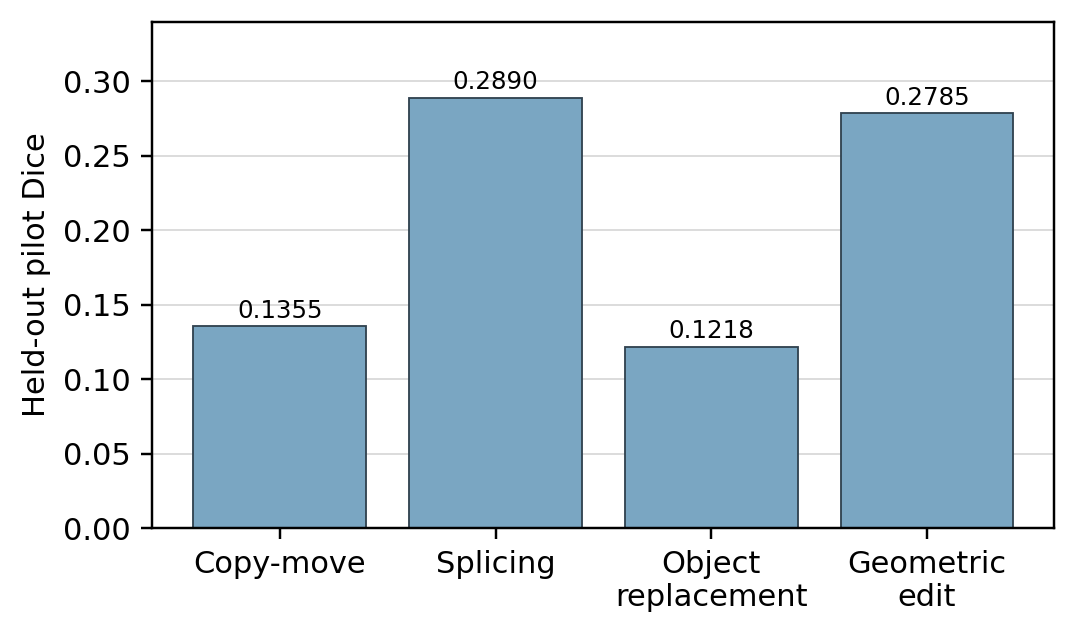
\includegraphics[width=0.92\linewidth]{pilot_by_manipulation.png}
  \caption{Held-out pilot Dice by manipulation type. The variation is a result, not an artifact to hide: the selected compression and resampling cues are not uniformly effective.}\label{fig:types}
\end{figure}

\begin{table}[t]
\caption{Held-out pilot Dice and mean detector time for 128$\times$128 images.}\label{tab:pilot}\small
\begin{tabular}{lcc}\toprule
Manipulation & Dice & N \\
\midrule
Copy-move & 0.1355 & 8 \\
Splicing & 0.2890 & 8 \\
Object replacement & 0.1218 & 8 \\
Geometric edit & 0.2785 & 8 \\
Overall & 0.2062 & 32 \\
\midrule
\multicolumn{3}{l}{Mean detector time (ms): SIFT 4.3; JPEG 11.4; resampling 98.4; block 7.7.}\\
\bottomrule\end{tabular}
\end{table}

\subsection{Public example and failure boundary}
Figure~\ref{fig:comofod} shows one official CoMoFoD original/forged pair and a pixel-difference view. The examples were downloaded from the official VCL site. They are useful for checking that public image content is readable by the pipeline, but the example page does not provide binary masks. They are therefore not used to claim localization accuracy.

\begin{figure}[t]
  \centering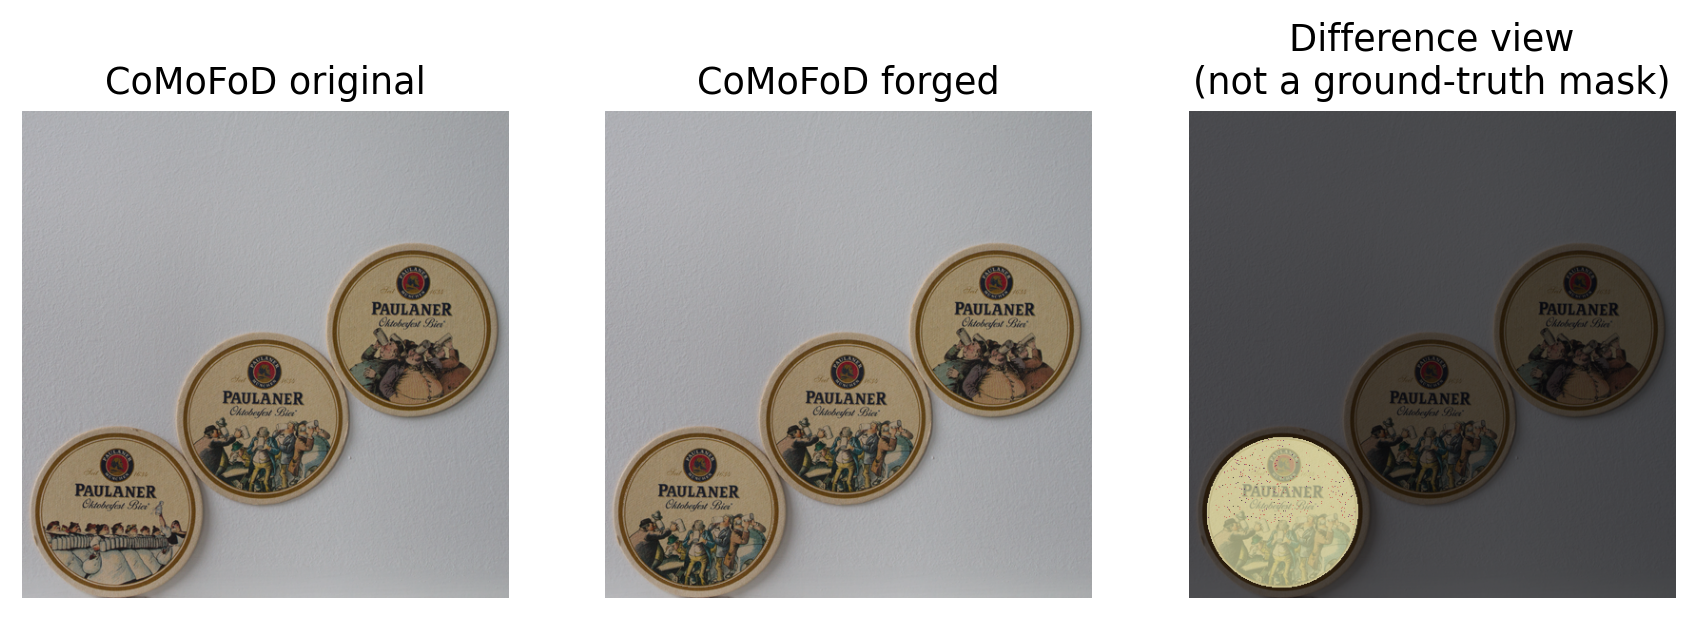
\includegraphics[width=\linewidth]{comofod_example.png}
  \caption{Official CoMoFoD example pair. The difference view is included for visual context only and is not a ground-truth mask. Quantitative evaluation requires the official binary mask files.}\label{fig:comofod}
\end{figure}

\subsection{Interpretation}
The pilot answers the procedural part of RQ2: a validation-only protocol can select a smaller subset when the full candidate pool ties it. It does not answer whether the subset is superior on natural public data. The pilot score is modest, and no confidence interval was estimated for this initial run. A publication-scale claim requires complete CoMoFoD or COVERAGE masks, paired uncertainty intervals, stress-condition results, and comparison with the strongest individual cue.

\section{Reproducibility and Engineering Constraints}
\subsection{Reproducibility record}
The repository records detector parameters, source identifiers, split assignments, cue availability, normalization statistics, weights, thresholds, runtime, and output maps. Public-source papers and provenance notes are stored in the references directory. Remote image or mask URLs are rejected by the manifest loader so that an evaluation cannot silently change when an external file changes.

\subsection{Engineering constraints}
The system uses classical image processing only and runs without a GPU. The design avoids learned fusion because the study asks which interpretable evidence domains add value. The main cost is the resampling cue, which is slower than the other candidates in the pilot. This cost is recorded so that a small gain cannot be treated as free.

\subsection{Threats to validity}
The pilot generator is not a natural-image benchmark. The JPEG cue is an approximation of the published JPEG-ghost procedure. The block cue is a heuristic and may be correlated with JPEG history. The public example images lack masks in the downloaded page. These limitations are explicit boundaries on the conclusions, not implementation details that can be ignored.

\section{Conclusion}
This paper presents a measurement protocol for selecting a small set of classical image-forensics cues. The candidate pool covers duplicated content, compression history, interpolation traces, and block-aligned anomalies. A validation-only pilot selected JPEG history, resampling, and block-grid evidence, but the held-out Dice score was modest and varied by manipulation type. The result supports the need for cue ablation and careful availability handling. It does not support a universal claim that the selected subset detects arbitrary tampering.

The next required experiment is a source-disjoint evaluation on the complete licensed CoMoFoD or COVERAGE release with binary masks, stress variants, and paired uncertainty intervals. Until that experiment is complete, the correct interpretation is a reproducible pilot and a defensible protocol for the final benchmark study.

\begin{acks}
The project follows the provided ACM manuscript template and section-by-section writing guide. Literature files and public examples are retained with provenance notes. No result is presented as a universal authenticity test.
\end{acks}

\bibliographystyle{ACM-Reference-Format}
\bibliography{references}
\end{document}
